%%%%%%%%%% Introduction %%%%%%%%%%
\chapter*{Linguistic peculiarities \\ \large The unusual vernacular of the Apocalypse}
  \markboth{Linguistic peculiarities}{Linguistic peculiarities}
  \addcontentsline{toc}{chapter}{Linguistic peculiarities}
  
\begin{wrapfigure}{R}{0.55\textwidth}
	\centering
	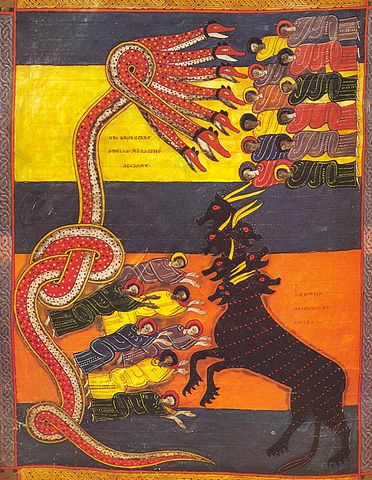
\includegraphics[width=0.5\textwidth]{images/linguisticpeculiarities/dragonsevenheads.jpg}
	\small\caption{The Dragon gives his power to the Beast — Facundus Beatus, 1047 AD}
\end{wrapfigure} 

Before we commence delving into the translation of the Apocalypse, I decided it would be of interest to showcase a handful of the key peculiarities of this particular book of the Bible. I will, thus, present to you those linguistic features I found noteworthy and explain the reasons behind my adding them here. 

I have been reading the Apocalypse of John — also known simply as Revelation in English — with great eagerness, as its subject matter easily makes it one of the most suspenseful books one can read in the New Testament. It is filled to the brim with colourful and intense imagery but also rather strange linguistic phenomena that appear to be rather unique to this particular author. Despite its being the last book of the New Testament, I find it is unparalleled in terms of actual content and makes for a most enjoyable read — its subject matter (i. e. the end of the world) notwithstanding.

I, thus, decided that it would be a rather interesting matter to explore in what manners this book shows its rather odd linguistic phenomena and what their reasons for existing might be. However, as I am, myself, not an expert on either this subject or the Ancient Greek language in general, I felt that it would be prudent to add a short disclaimer here, stating that any of the below-mentioned opinions and observations may turn out to be utterly false. Should I, over the course of the next few weeks, months and years, be corrected, I will amend the pages as needed and promptly publish an updated edition of my book. 

Please also note that all the translations of Greek passages you will find below are going to be either taken from the NKJV or YLT unless otherwise stated. Their origin will, nevertheless, be clearly marked within parentheses.

\section*{An unfortunate circumstance}
  \addcontentsline{toc}{section}{An unfortunate circumstance}
  
Indeed, his often rather unusual — and, at times, even entirely incorrect — usage of the Greek language and its grammar has lead many people to claim that the his prose is outright bad. I had asked a question on a forum regarding the language used in the Revelation and wanted to know whether it was as bad as so many people are claiming it to be; and I received rather varied replies. This was before I had begun reading it and the only things I had heard about it at the time were complaints regarding its low-quality prose.

Because of this, I had been putting off reading the Apocalypse, as I had been deeming it unworthy of my time to read such a lowly piece of text — for, truly, what would be the point in reading a text if, at worst, it will simply degrade your Greek? Nevertheless, the fact that it is is included in the canon of the New Testament is what finally made me realise that the early Christians must have thought it a text worthy to be included — a judgement that not many other texts have passed. I, thus, set aside my prejudice — the one which I received by reading the very vocal opinions of others online — and simply began reading; and, lo and behold, its grammatical quirks are completely overshadowed by its suspenseful and intriguing subject matter.

\begin{wrapfigure}{R}{0.55\textwidth}
	\centering
	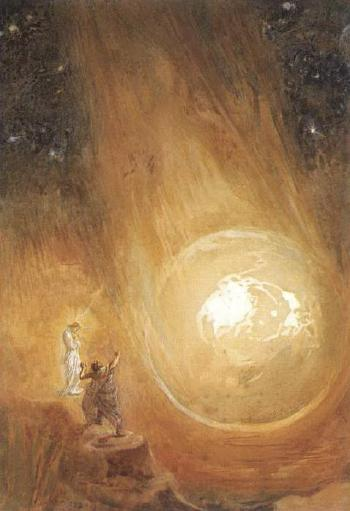
\includegraphics[width=0.5\textwidth]{images/linguisticpeculiarities/fallenstar.jpg}
	\small\caption{And I saw a Star fall from Heaven — Henry John Stock, 1902}
\end{wrapfigure} 

Therefore, in addition to the simple desire of explaining and analysing aforesaid quirks, I am writing the following text in the hopes that people might be able to look past its strange and sometimes incorrect composition and see it for what it is: a brilliantly — albeit not eloquently — composed text written by a non-native speaker of the Greek language. And because his personal, linguistic traits have not been (entirely) rewritten by the subsequent copiers of his works in an effort to correct his work, we can, in turn, gain a unique insight into the person who wrote the last book of the New Testament.

Indeed, I should begin with a short explanation of aforesaid linguistic phenomena. Ancient Greek, as any language, has a set of rules which govern how the language functions, called grammar. A diversion from said rules will either lead to misunderstanding or no understanding at all; but if aforementioned diversion is one that is not too great, it can, often-times, still be understood by the reader — and the latter is what we find in the Apocalypse of John.

His writing is filled with such peculiarities, all of which fall under one of two (and sometimes both) categories: grammatically incorrect but still understandable; and grammatically correct but not the typical manner in which a native Greek speaker would have written it (though the latter might, by some, also be regarded as technically grammatically incorrect).

Into the former category fall things which are plainly wrong and which the majority of people would regard as such, as, for example, the misuse of grammatical gender. The latter category mainly includes things which were coloured — so to speak — by the author’s native Semitic language but which, I would argue, can still be counted as technically grammatically correct.

I am certain that a number of people will disagree with me on this regard — and I encourage them to, especially considering my comparative lack of exposure to Ancient Greek materials —, but I, nonetheless, find this classification of linguistic quirks in the Revelation fitting. And whilst I do believe that a more fine-tuned classification — which takes into consideration more of the minutiæ of the prose — would have been possible, I did not believe that such a detailed description of linguistic peculiarities was necessary in a short article such as this one.

\section*{ὁ ὢν καὶ ὁ ἦν καὶ ὁ ἐρχόμενος}
  \addcontentsline{toc}{section}{ὁ ὢν καὶ ὁ ἦν καὶ ὁ ἐρχόμενος}
  
The extract above showcases one of the strange grammatical features of John’s Revelation. The NKJV of the New Testament renders it as follows: “[…] who is and who was and who is to come […]”; and, indeed, this is also how I had come to understand this phrase, which occurs numerous times over the course of the book. I find the usage of the present participle somewhat strange, however, and am at a loss as to why ὤν (lit. “being”) was chosen as opposed to the regular ἐστίν (lit. “is”). The participle here is in stark contrast, I find, to the then following imperfective ἦν (lit. “was”).

If I were to guess the reason behind his choosing the participle instead of the actual, conjugated verb — especially considering the fact that the author knew of the existence of the 3rd person singular, present active indicative form of εἰμί (namely ἐστίν) and uses it frequently —, I would postulate that it was chosen to convey the meaning of continuous being.

This is due to the fact that the action described by a present participle is generally contained within the exact same temporal frame as the main verb — and when there is not a main verb which the participle refers to, I find that, frequently, the present participle is used in a similar fashion to that of the English language. This is to say that Greek — in the form used in the Septuagint and the New Testament, at least — frequently uses the present participle to convey something similar to the English continuous or progressive aspects (i. e. the difference in meaning between I run and I am running).

Thus, the sentence could, perhaps, also be translated as “Who is being …”; though, as stated previously, I am uncertain as to whether or not this assertion is correct, mainly due to my still rather limited knowledge of Greek literature. Nevertheless, I would classify this as a peculiarity rather than a grammatical mistake; if anything, it adds to the often very colourful language of the Apocalypse.

\section*{ἐδόθη αὐτῷ}
  \addcontentsline{toc}{section}{ἐδόθη αὐτῷ}

Another comparatively unique feature of John’s writing is the frequent usage of a particular form of the divine passive; this appears to be the name given to this particular usage of the Greek passive by a surprisingly large amount of people online. Indeed, simply typing in the words “divine pas …” into Google will automatically yield the following search suggestion: “divine passive Greek”. There appear to be a good number of various forum and blog posts regarding this particular subject which is, by no means whatsoever, entirely unique to the Apocalypse. Nevertheless, John’s frequent usage of the expression ἐδόθη αὐτῷ ([it was] given to him) — or variants thereof — is most definitely interesting and warrants the taking of a closer look at it.

The divine passive is less of an actual grammatical phenomenon and rather a theological one; its meaning is still that of a passive (“given to him”) but the implied agent — i. e. the person who is the active participant of the passive verb — is God. The Christians of the time — which, most likely, would have still called themselves Jews — were not very keen on using the Lord’s name if they could at all avoid it. This avoidance was so far reaching that the pronunciation of the very-well known Tetragrammaton יהוה‎ (YHWH) gradually became lost over the course of history, simply due to people avoiding to utter it. Thus, instead of referring to the Lord by his proper name Yahweh — which is the modern reconstructed and generally agreed upon pronunciation of his name —, the Jews of the time preferred to refer to Him using either אֲדֹנָי‎ (adonai, My Lord) or אֱלֹהִים‎ (elohim, God(s)).

It should, therefore, not be surprising that when a passive was used whose agent was easily understood as being God Himself, the author did not wish to include His name if it was not, at all, necessary. This particular divine passive — namely ἐδόθη αὐτῷ — enjoys a large usage in the Revelation and is, I would argue, most frequently used in reference to both items and (supernatural) powers which were given by Him to the various actors of the Apocalypse. The following is a passage from Rev. 9:1: —

\begin{quote}

\textbf{GRC}: Καὶ ὁ πέμπτος ἄγγελος ἐσάλπισεν· καὶ ἴδον ἀστέρα ἐκ τοῦ οὐρανοῦ πεπτωκότα εἰς τὴν γῆν, καὶ ἐδόθη αὐτῷ ἡ κλεὶς τοῦ φρέατος τῆς ἀβύσσου. 

\textbf{Transliteration}: Kai ho pemptos angelos esalpisen; kai idon astera ek tou ouranou peptōkota eis tēn gēn, kai edothē autō hē kleis tou phreatos tēs abyssou. 

\bigskip

\textbf{NKJV}: Then the fifth angel sounded: And I saw a star fallen from heaven to the earth. To him was given the key to the bottomless pit. 

\textbf{YLT}: And the fifth messenger did sound, and I saw a star out of the heaven having fallen to the earth, and there was given to it the key of the pit of the abyss.
\end{quote}

The key being given to the being so colourfully represented by a fallen star — namely Satan — was given by an actor that has not been called by name; the key was simply given. Such examples of the aforementioned divine passive are plentiful within in the Apocalypse of John, and his particular affinity for the phrase ἐδόθη αὐτῷ — and its derivatives — is both interesting and unusual; truly, someone not used to the usage of the passive in this way will, undoubtedly, be quite confused.

But, as previously mentioned, this construction is not only used for physical things handed by God to certain people, but even (supernatural) powers or general authorities. An example of this can be found in Rev. 6:4, where it says that “ἐδόθη αὐτῷ λαβεῖν τὴν εἰρήνην ἐκ τῆς γῆς (edothē autō labein tēn eirēnēn ek tēs gēs)” which can be literally translated as “It was given to him to take the peace from the Earth.” It is, however, plainly obvious that an exchange of physical goods did not take place in this passage; instead, He granted the person riding the horse the power to take the aforementioned peace from Earth.

I personally find this an interesting usage of the passage and a rather creative way of avoiding having to write the Lord’s name.

\section*{Usage of the nominative after a declined word}
  \addcontentsline{toc}{section}{Usage of the nominative after a declined word}
  
 Another strange feature is his frequent usage of the nominative following a noun declined in a different case. For example, in Rev. 1:5, the following sentence can be found: “καὶ ἀπὸ Ἰησοῦ Χριστοῦ, ὁ μάρτυς ὁ πιστός (kai apo Iēsou Christou, ho martys ho pistos).” Herein, a genitive noun — Ἰησοῦ Χριστοῦ, lit. of Jesus Christ — is followed by another noun and an adjective — both of which refer to aforementioned genitive — declined not in the genitive case, but in the nominative.

\begin{wrapfigure}{R}{0.55\textwidth}
	\centering
	
\includegraphics[width=0.5\textwidth]{images/linguisticpeculiarities/fugelangelfromheaven.jpg}
	\small\caption{He laid hold of the dragon, that serpent of old, who is the Devil and Satan, and bound him for a thousand years (Rev 20:1) — Gebhard Fugel, 1933}
\end{wrapfigure}

Thus, the grammatically correct form of this passage would be “καὶ ἀπὸ Ἰησοῦ Χριστοῦ, τοῦ μάρτυρος τοῦ πιστοῦ (kai apo Iēsou Christou, tou martyros tou pistou)”, wherein the adjective and noun, following Jesus’ name declined in the genitive, are, too, declined in the genitive case.

Indeed, other languages with grammatical cases and gender, such as German, do the exact same thing, albeit in the dative rather than the genitive in this particular instance: “und von Jesu Christo, dem Zeugen dem treuen […]” instead of “[…] der Zeuge der treue”. Nevertheless, German could, potentially, render the following noun and adjective in the nominative if the sentence were changed slightly, such as can be found in the Einheitsübersetzung 2016: “und von Jesus Christus; er ist der treue Zeuge”, lit. and from Jesus Christ; he is the loyal witness.

This leads me to believe that this might have been John’s intention after all and he simply forgot to — or did not wish to — place the additional words into his sentence which would have rendered the nominative a valid form; though, once more, I cannot be entirely certain.

However, in the beginning of the 19th century, a Greek cleric and educator named Νεόφυτος Βάμβας (Neophytos Vamvas) decided to translate the Bible into the then modern variant of Greek; and, surprisingly, in his translation, the grammatical error is corrected insofar that he actually does add the words necessary to have the words following the genitive form of Jesus Christ be in the nominative: “και από του Ιησού Χριστού, όστις είναι ο μάρτυς ο πιστός (kai apó tou Iisoú Christoú, óstis eínai o mártys o pistós)” — his translation can be translated as “and from Jesus Christ, who is the witness, the loyal (one).”

\section*{Inconsistent tense usage}
  \addcontentsline{toc}{section}{Inconsistent tense usage}

\section*{Conclusion}
  \addcontentsline{toc}{section}{Conclusion}
  
To conclude this short introduction to John's peculiar way of writing — and, perhaps, speaking —, we can safely say that, even though his style is most unusual indeed, it rarely leaves one mystified as to the intention of the writer. And whilst he does make frequent grammatical mistakes and writes a lot of things in a rather atypical fashion, I personally find that this is precisely what makes the Apocalypse such an interesting text to read.


  